% !TEX encoding = UTF-8 Unicode
\section{Der Editor}
\subsection{Die Bühne}
Die ''Bühne'' macht den größten Teil des Editors aus. Auf ihr können Plugins, Module sowie Regler platziert und bedient werden.
\subsection{Die Mauskontext-Auswahl}
Oben links im Editor befindet sich die Mauskontext-Auswahl: 
\includegraphics[scale=0.5]{../graphics/mousecontext}. Der gewählte Mauskontext bestimmt, in welcher Art und Weise, auf der Bühne befindliche Elemente benutzt werden können:
\\
\begin{description}
	\item[Benutzen]  (
\includegraphics[scale=0.5]{../graphics/muse}) Um Elemente wie Drehregler auf der Bühne zu bedienen, wählen Sie den ''Benutzen''- Kontext.
	\item[Verbinden] (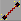
\includegraphics[scale=0.5]{../graphics/mconnect}) ist ''Verbinden'' gewählt, können zwei Elemente mit der Maus verbunden werden. Klicken Sie dabei auf das erste Element und ''ziehen'' Sie den Mauszeiger auf das zweite Element. Sind beide Elemente verbindbar, wird die soeben erstellte Verbindung durch eine Linie dargestellt.
	\item[Bewegen]   (
\includegraphics[scale=0.5]{../graphics/mmove}) Jedes Element auf der Bühne ist verschiebbar: wählen Sie ''Verschieben'', klicken Sie auf ein Element und ziehen Sie es an eine beliebige Position. Ausserdem lässt sich mittels ''Verschieben''-Kontext die Bühne selbst verschieben. Klicken Sie hierfür auf eine Position der Bühne, an dem sich kein Element befindet und ziehen Sie Maus in eine beliebige Richtung.
\end{description}

\subsection{Das Hauptmenü}
\begin{figure}[htbp]
\begin{center}
	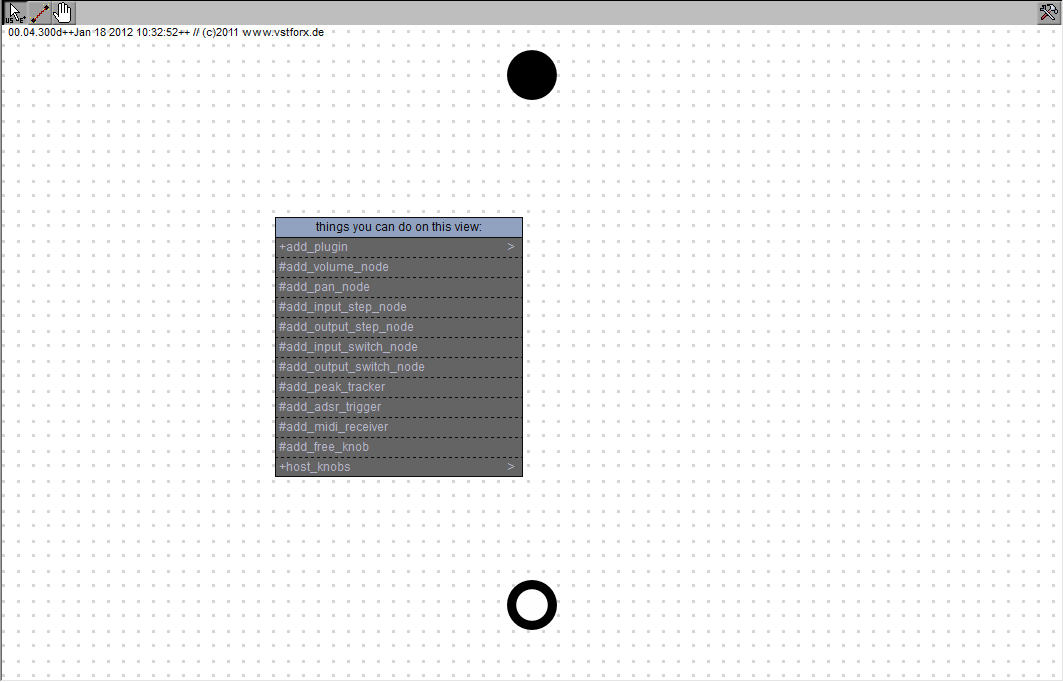
\includegraphics[scale=0.5]{../graphics/main_menu}
\caption{Das Hauptmenü}
\label{main_menu}
\end{center}
\end{figure}

VSTForx wird Hauptsächlich durch ein Kontextmenü gesteuert. Je nachdem, an welcher Position auf der ''Bühne'' Sie das Kontextmenü aufrufen ( unter Windows ist das Standardmäßig die Rechte Maustaste, unter Mac: ''Ctrl + Maustaste'' ) werden Unterschiedliche - zum Bühnenobjekt - passende Menüpunkt aufgezeigt.
Das Hauptmenü können Sie öffnen, indem Sie an einer leeren Stelle der ''Bühne'' das Kontextmenü aufrufen (siehe Abbildung \ref{main_menu}). 
\\\\
Folgende Aktionen können Sie mit dem Hauptmenü ausführen:
\paragraph{ein Plugin hinzufügen}
\untermenupunkt{add\_plugin}
\paragraph{ein Lautstärke Modul hinzufügen}
\menupunkt{add\_volume\_node}
\paragraph{ein Pan Modul hinzufügen}
\menupunkt{add\_pan\_node}
\paragraph{ein Eingangs-Step Modul hinzufügen} 
\menupunkt{add\_input\_step\_node}
\paragraph{ein Ausgangs-Step Modul hinzufügen}
\menupunkt{add\_output\_step\_node}
\paragraph{ein Peak Tracker Modul hinzufügen}
\menupunkt{add\_peak\_tracker}
\paragraph{ein ADSR Trigger Modul hinzufügen}
\menupunkt{add\_adsr\_trigger}
\paragraph{ein Midi Tracker Modul hinzufügen}
\menupunkt{add\_midi\_tracker}
\paragraph{ein Drehregler hinzufügen}
\menupunkt{add\_free\_knob}
\paragraph{ein Host-Drehregler hinzufügen}
\untermenupunkt{host\_knobs}











